\documentclass[abstracton,12pt]{scrreprt}

\usepackage[utf8]{inputenc}
\usepackage[T1]{fontenc}
\usepackage{fancyhdr}
\usepackage{graphicx}
\usepackage{tikz}
\usepackage{times}
\usepackage{listings}
\usepackage{amssymb}
\usepackage{amsfonts}
%\usepackage{algorithm}
\usepackage{algpseudocode}
\usepackage{mathtools}
\usepackage{amsmath}
\usepackage{url}
\usepackage{chapterbib}
\usepackage{gensymb}
\usepackage{BTree}
\usepackage{weiwBTree}
\usepackage{float}
\usepackage{array}
\usetikzlibrary{shapes, calc}
\usepackage[ruled,linesnumbered,lined,commentsnumbered]{algorithm2e}

\setlength{\parindent}{0pt} 


\titlehead{Department of Informatics, University of Zürich}
\subject{\vspace*{2cm}BSc Thesis}
\title{Implementing an Index Structure for Streaming Time Series Data}
\author{
  Melina Mast\\[-5pt]
  \scriptsize Matrikelnummer: 13-762-588\\[-5pt]
  \scriptsize Email: \texttt{melina.mast@uzh.ch}
}
\date{\vspace*{2cm}August, 2016}
\publishers{
  \small supervised by Prof.\ Dr.\ Michael Böhlen and Kevin Wellenzohn \\[5cm]
  \begin{tikzpicture}[overlay]
    \node at (-3,-3) {
\includegraphics[height=5.5cm]{IFIlogo}};
    \node at (7,-3) {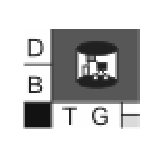
\includegraphics[height=2cm]{dbtgBW}};
  \end{tikzpicture}
}

%----\dedication{dedicated to xxx}

% --------- 

\newtheorem{definition}{Definition}
\newtheorem{example}{Example}
\newtheorem{theorem}{Theorem}
\newtheorem{lemma}{Lemma}

\newenvironment{proof}
  {\noindent{\bf Proof:\rm}}{\hfill$\Box$\vspace{\medskipamount}}

\def\bbbr{{\rm I\!R}}
\def\bbbm{{\rm I\!M}}
\def\bbbn{{\rm I\!N}}
\def\bbbz{{\rm I\!Z}}

% --------- 

\begin{document}


\maketitle

\chapter*{Acknowledgements}



\begin{abstract}
  ...
\end{abstract}

\chapter*{Zusammenfassung}

\tableofcontents
\listoffigures
\listoftables
\listofalgorithms
\renewcommand{\lstlistingname}{Algorithm}% Listing -> Algorithm


\addtocontents{loa}{\def\string\figurename{Algorithm}}

\chapter{Introduction}

The thesis presents a way to implement the described data structures after discussing the requirements. Furthermore, it documents the out coming experimental results.
In the end of the thesis, in Chapter \ref{sec:Summary}, the findings will be summarized and concluded.

\section{Thesis Outline}


\newtheorem{defn}{Definition}[section]
\newtheorem{exmp}{Example}[section]
\newcommand*{\argmin}{\operatornamewithlimits{argmin}\limits}

\chapter{Background}
\label{background}
A streaming time series $s$ is a unbounded sequence of data points that is continuously extended, potentially forever. Streaming time series are relevant to applications in diverse domains for example in finance, meteorology or sensor networks. All domains have applications that need to be fed continuously with the latest data e.g. the financial stock market or the weather information. But the processing of large volumes of time series data is impractical. Therefore, a system can only keep a limited size of data in main memory.\\
The data that is kept in main memory needs to be limited to just a portion of the streaming time series. Besides, in order to be practical for a application like the financial stock market, the data that arrives in a defined time interval (e.g. every 2 minutes) needs to be completely processed until the succeeding data arises.

\section{TKCM}
A streaming time series is not always gapless. E.g due to sensor failures or transmission error, values can get missing. Wellenzohn et al.\cite{BScT} presents a two-dimensional query pattern over the most recent values of a set of time series to efficiently impute missing values. The two-dimensional query pattern $P_{\bar{t}}$ is defined with \emph{l} reference time series on the spatial dimension and a time window of length \emph{p} on the time dimension. The idea is to derive the missing value from the \emph{k} most similar past pattern. Therefore, it determines for each \emph{time series} a set of highly correlated \emph{reference time series} which represent similar situations in the past e.g. similar weather situations. The value $\hat{s}(t)$ that is calculated as the average of the values $\{s(t) | t \in T_k\}$ will be imputed. Hence, TKCM is able to calculate an estimation of a missing value in streaming time series data. \\ \\
TKCM must not only insert missing values, but also process the newest arriving values efficiently. In order to do that, TKCM must provide an insertion method for new arriving values to insert the new value into the time window $W$. Since the time window has a limited, given size $|W|$, an old value has to be deleted for the new arriving value. Provided that, the oldest time \emph{t} does no more fit into the time window because the window is already full. \\
Further, TKCM must be able to handle duplicate values. For example, if the time window contains 100 temperature values from the same weather station and every 5 minutes a new value arrives. It is likely that the same temperature value arrives multiple times. 
Besides, the most similar base time values for a given value \emph{v} should be efficiently found and returned.\\
These assumptions can be made for the implementation of the index structure for streaming time series data.


\section{Access Methods}
\label{AccessMethods}
TKCM initializes a set $T =\{\}$. The set is filled during execution with all time points \emph{t} for which pattern $P_t$ has already been compared to the query pattern $P_{\bar{t}}$. Besides, TKCM initializes a set $T^*=\{\}$ that contains the \emph{k} time points $t \in T$ that minimize the error $\delta(P_{t}, P_{\bar{t}})$. Therefore, $T^* \subseteq T$ is always true during execution. 
\\TKCM uses two methods for accessing any time series $r \in S$, \emph{random} and \emph{sorted} access. The two methods are defined as follows: 
\begin{defn}
	Random Access. Random access returns value r(t), given time series r and time point t.	
\end{defn}
\begin{defn}
	Sorted Access. Sorted access returns the next yet unseen time point $t_s \notin T$ such that the value $r(t_s-o)$ is most similar to a given pattern cell $P_{\bar{t}}^{r,o}$. $t(s)$ is defined as:
	\begin{align*}
	t_s = \argmin_{t_s \in W \setminus T} |r(t_s-o) - P_{\bar{t}}^{r,o}|
	\end{align*}
\end{defn}
After $T$ and $T^*$ is initialized, TKCM iterates until set $T^*$ contains the $k$ time points $t$ that minimize the difference $\delta(P_{t}, P_{\bar{t}})$. \\Using the sorted access mode, the algorithm loops through the cells $P_{\bar{t}}^{r,o}$, reading the next potential time point $t_s \notin T$. The time point $t_s \notin T$ is added to $T$. The time point $t_s$ has a corresponding patter $P_{t_s}$ which is at least for one pattern cell similar to the query pattern $P_{\bar{t}}$. \\
The random access mode is used to look up the values that pattern $P_{t_s}$ is composed of. After each iteration a threshold $\tau$ is computed. The threshold $\tau$ is a lower-bound on the error $\delta (P_{t^{'}}, P_{\bar{t}})$ for any time point $t^{'}$ that is yet unseen. Therefore, during the execution of the algorithm
$\forall t^{'} \in T : \tau \leq \delta(P_{t^{'}}, P_{\bar{t}}) $ is valid. Informally this significances that the lower-bound is always smaller or equal to the error between pattern $P_{t^{'}}$ and query patter $P_{\bar{t}}$ for all time points $t^{'}$ that are elements of $T$. Once $\forall t \in T^* : \delta(P_{t}, P_{\bar{t}}) \leq \tau$ the algorithm terminates. At the end, $T^*=T_k$.

\chapter{Problem Definition}
The present thesis tries to introduce an efficient way to implement the $random$ and $sorted access$ methods described in Section \ref{AccessMethods} for a streaming time series $s$.\\
Let $W=[ \underline{t}, \bar{t} ]$ be a sliding window of length $|W|$. Time $\underline{t}$ stands for the oldest time point that fits into the time window and $\bar{t}$ stands for the current time point for which the stream produced a new value. Besides, consider a set $S = \{s_1,s_2,...\}$ of streaming time series. The value of time series $s \in S$ at time \emph{t} is denoted as $s(t)$. Only the values in the time window $W$ are kept in main memory. However, we assume that all the time points $t < \bar{t}$ have a time series \emph{s} that is complete. Hence, $\forall t < \bar{t} : s(t) \ne NIL$ since \emph{s} contains imputed values if the real ones were missing. 

\section{Operations}
\label{sec:Op}
The system presented in the present thesis needs to efficiently perform on the streaming time series $s$ in a sliding window $|W|$: 
\begin{itemize}  
	\item shift$(\bar{t}, v)$: add value \emph{v} for the new current time point $\bar{t}$ and remove value \emph{v'} for the time point $\underline{t} - 1$ that just dropped out of time window $W$.
	\item lookup$(t)$: return the value of time series \emph{s} at time \emph{t}, denoted by $s(t)$.
	\item neighbor$(v, T)$: given a value \emph{v} and a set of time points $T$, return the time point $t \in T$ such that $|v-s(t)|$ is minimal.
\end{itemize}
The $lookup$ operation is a random access method, while the $neighbor$ operation is a sorted access method.\\
Wellenzohn et al.\cite{BScT} suggests a combination of two data structures: a $B^+$ tree and a circular array. The lookup operation can be performed by the circular array, while the neighbor operation takes advantage of the fact that the leaves of a $B^+$ tree are sorted.\\
The approach presented in in Chapter \ref{sec:Approach} the implementation of the random and sorted access modes using the suggested data structures. Further, it proposes a solution to handle duplicate values. 


\chapter{Approach}
\label{sec:Approach}
The lookup operation can be efficiently performed by the circular array, while the neighbor operation takes advantage of the fact that the leaves of a $B^+$ tree are sorted. \\
Each time series $s \in S$ can be implemented as a circular array. The circular array is kept in main memory. It uses random access to look up value $s(t)$ for a given time $t$. Further, for each time series $s$ a $B^+$ tree is maintained that is also kept in main memory. The $B^+$ tree is ideal for sorted access by value and therefore for range queries. Both data structures are described in detail in Section \ref{sec:circularArray} and Section \ref{sec:BplusTree}.


\section{Circular Array}
\label{sec:circularArray}
A circular array is used to store the time series data. The data is assorted by time. Further, the time interval is predefined e.g. every 5 minutes a new value arrives.\\ The value and time are directly stored in the circular array. The last update position is stored in a variable and updated with every insertion. The circular array is shown in Figure \ref{fig:cat}.\\
\begin{figure}[htbp]
	\centering
	\begin{tikzpicture}[
	scale=0.7,
	every node/.style={outer sep=0pt, transform shape, font=\scriptsize},
	every matrix/.style={cells={scale=0.7}},
	]
	
	% circular array
	\xyshift{-15mm}{-70mm}{
		\matrix [ampersand replacement=\&, outer sep=0pt, matrix anchor=north] (array) {
			\node[circularptr] (c1)  {3.2}; \&
			\node[circularptr] (c2)  {1.3}; \&
			\node[circularptr] (c3)  {4.5}; \&
			\node[circularptr] (c4)  {4.6}; \&
			\node[circularptr] (c5)  {6.2}; \&
			\node[circularptr] (c6)  {3.2}; \&
			\node[circularptr] (c7)  {11.2}; \&
			\node[circularptr] (c8)  {55.3}; \&
			\node[circularptr] (c9)  {9.1}; \&
			\node[circularptr] (c10) {3.9}; \&
			\node[circularptr] (c11) {5.0}; \&
			\node[circularptr] (c12) {1.4};  \\
			%
			\node[circularval] (left) {14:10}; \&
			\node[circularval] {14:15}; \&
			\node[circularval] {14:20}; \&
			\node[circularval] {14:25}; \&
			\node[circularval] {13:30}; \&
			\node[circularval] {13:35}; \&
			\node[circularval] {13:40}; \&
			\node[circularval] {13:45}; \&
			\node[circularval] {13:50}; \&
			\node[circularval] {13:55}; \&
			\node[circularval] {14:00}; \&
			\node[circularval] (right){14:05};\\
		};
	}
	% curly brace
	\draw [decorate,decoration={brace,mirror,amplitude=10pt}]
	([yshift=-5pt] left.south west) -- ([yshift=-5pt] right.south east)
	node [black,midway,yshift=-0.9cm] {\large size $|W|$};
	\end{tikzpicture}
	\vspace{2mm}
	\caption{Circular array of size $|W|$.}
	\label{fig:cat}
\end{figure}\\
The circular array stores the data, containing all measurement time stamps and values, the size, the last update Position and a counter, which counts the number of measurements added to the array. The addition of a new measurement to the array is presented in Algorithm \ref{alg:Update Circular Array}.


\newpage
\section{$B^+$ Tree}
\label{sec:BplusTree}
A $B^+$ tree is able to execute range queries very efficiently, since the leaves of a $B^+$ tree are ordered and linked. To perform the \emph{neighbor}$(v,T)$ operation described in Section \ref{sec:Op}, the $B^+$ tree for our requirements has leaves linked in both directions. The Section \ref{structureBtree} presents the structure of the $B^+$ tree we used for the implementation.
\begin{figure}[htbp]
	\centering
	\begin{tikzpicture}[
	scale=0.7,
	every node/.style={outer sep=0pt, transform shape, font=\scriptsize},
	every matrix/.style={cells={scale=0.7}},
	]
	% root node
	\xyshift{-20mm}{0mm}{\btreeinodethree{root}{17}{}{}};
	
	%
	% intermediate nodes
	\xyshift{-50mm}{-15mm}{\btreeinodethree{n1}{7}{}{}{}}
	\xyshift{ 10mm}{-15mm}{\btreeinodethree{n2}{23}{37}{43}}
	%
	% connecting root to intermediate level nodes
	\foreach \x in {1,2} { \btreelink{root-\x}{n\x} }
	%
	% leaf nodes
	\xyshift{-90mm}{-30mm}{\btreelnodethree{n11}{2.5}{3}{6.1}}
	\xyshift{-60mm}{-30mm}{\btreelnodethree{n12}{7}{13.2}{}}
	\xyshift{-30mm}{-30mm}{\btreelnodethree{n21}{17}{18.1}{}}
	\xyshift{ 0mm}{-30mm}{\btreelnodethree{n22}{23}{25.4}{}}
	\xyshift{ 30mm}{-30mm}{\btreelnodethree{n23}{37}{38.9}{40}}
	\xyshift{ 60mm}{-30mm}{\btreelnodethree{n24}{43}{47.1}{}}
	%
	% connecting intermediate level to leaf nodes
	\foreach \x in {1,2}     { \btreelink{n1-\x}{n1\x} }
	\foreach \x in {1,2,3,4} { \btreelink{n2-\x}{n2\x} }
	%
	% leaf pointers
	\draw[btlink] ([yshift=+3pt] n11-c.east) -- ([yshift=+3pt] n12-a.west);
	\draw[btlink] ([yshift=-3pt] n12-a.west) -- ([yshift=-3pt] n11-c.east);
	\draw[btlink] ([yshift=+3pt] n12-c.east) -- ([yshift=+3pt] n21-a.west);
	\draw[btlink] ([yshift=-3pt] n21-a.west) -- ([yshift=-3pt] n12-c.east);
	\draw[btlink] ([yshift=+3pt] n21-c.east) -- ([yshift=+3pt] n22-a.west);
	\draw[btlink] ([yshift=-3pt] n22-a.west) -- ([yshift=-3pt] n21-c.east);
	\draw[btlink] ([yshift=+3pt] n22-c.east) -- ([yshift=+3pt] n23-a.west);
	\draw[btlink] ([yshift=-3pt] n23-a.west) -- ([yshift=-3pt] n22-c.east);
	\draw[btlink] ([yshift=+3pt] n23-c.east) -- ([yshift=+3pt] n24-a.west);
	\draw[btlink] ([yshift=-3pt] n24-a.west) -- ([yshift=-3pt] n23-c.east);
	%
	
	\foreach \x in
	{n11-1, n11-2, n11-3,n12-1, n12-2,n21-1,n21-2,n22-1, n22-2, n23-1, n23-2, n23-3, n24-1,n24-2}
	{ \path[<-] ([yshift=-15pt] \x.center) edge ([yshift=2pt] \x.center); }
	%
		

	\end{tikzpicture}
	\vspace{2mm}
	\caption{Example of a $B^+$ tree}
	\label{fig:BTreeBook}
\end{figure}


\subsection{The Structure of the used $B^+$ tree}
\label{structureBtree}
The structure of the used $B^+$ tree and its implementation is based on the book of Silberschatz et al.\cite{DatabaseSystemC}. \\
The difference to the traditional $B^+$ tree and our used $B^+$ tree is on the one hand, that the leaves are linked to the succeeding as well as the preceding leaf to efficiently perform the \emph{neighbor}$(v,T)$ operation and on the other hand, that the $B^+$ tree is constructed to handle duplicate values. How our tree handles duplicate values is described in Section \ref{sec:allowDV}. The other properties of our $B^+$ tree are presented in the following paragraph.\\ \\
A $B^+$ tree is organized in blocks. All paths from the root to a leaf in a $B^+$ tree have the same length. This significances that the tree is always \emph{balanced}. The balanced property ensures good performance for lookup, insertion and deletion that is why we use a $B^+$ tree. The $shift$ and the $neighbor$ operation are operations on the $B^+$ tree.\\There are three types of nodes that may exist in a $B^+$ tree: the root, interior nodes and leave nodes. The parameter \emph{n} determines the number of search-keys and pointers in a node. The interior nodes can have maximum \emph{n-1} search-keys and \emph{n} pointers, pointing to its child nodes. \\
A leaf node must have at least $[(n-1)/2]$ keys and may hold up to $n-1$ keys.\\
The structure of nonleaf nodes like interior nodes and the root, is the same as for leaf nodes. Except
for the pointers which points to tree nodes. An interior node must have a minimum of $[n/2]$ pointers. Hence, it must have a minimum of $[n/2]-1$ keys and can hold up to $n$ pointers. \\
The root node is the only node that can contain less than $[n/2]$ pointers. The root node must have minimum one searchkey and two pointers to child nodes, unless the root node has no children and therefore is a leaf node.
\begin{example}
	If $n$ is set to 7, an internal node may have between 4 and 7 children and therefore between 3 and 6 keys. The root may have between 2 and 7 children or if it is the only node in the tree it can have no children and just 1 key. A leaf node must have at least 3 keys and can have maximum 6 keys.
\end{example}
A node containing $m$ pointers $\left(m \leq n\right)$. For $i = 2, 3, . . . ,m-1$, pointer $P_i$ points to the subtree that contains searchkey values less than $K_i$ and greater than or equal to $K_{i-1}$. Pointer $P_m$ points to the part of the subtree that contains those key values greater than or equal to $K_{m-1}$. The searchkeys in the leaves are sorted from left to right. 
\begin{figure}[ht!]
	\centering
	\begin{tikzpicture}[
	scale=0.7,
	every node/.style={outer sep=0pt, transform shape, font=\scriptsize},
	every matrix/.style={cells={scale=0.7}},
	]
	% root node
	\xyshift{-20mm}{0mm}{\btreeinodethree{root}{17.2}{}{}};
	
	%
	% intermediate nodes
	\xyshift{-50mm}{-15mm}{\btreelnodethree{n1}{7.5}{16.4}{}{}}
	\xyshift{ 10mm}{-15mm}{\btreelnodethree{n2}{17.2}{33.1}{43.5}}
	%
	% connecting root to leaf level nodes
	\foreach \x in {1,2} { \btreelink{root-\x}{n\x} }
	%
	% leaf pointers
	\draw[btlink] ([yshift=+3pt] n1-c.east) -- ([yshift=+3pt] n2-a.west);
	\draw[btlink] ([yshift=-3pt] n2-a.west) -- ([yshift=-3pt] n1-c.east);
	%
	\end{tikzpicture}
	\vspace{2mm}
	\caption{Left children keys < 17.2 and right children keys $\geq$ 17.2}
	\label{fig:BTreeBook}
\end{figure} 
\\A value in the time window $W$ can occur multiple times. Hence, the values are not unique. Since the values are used as search-keys, the $B^+$ tree must be able to handle duplicate values. Section \ref{sec:allowDV} proposes our approach that allow to use duplicate values in a $B^+$ tree. 

\section{Handling Duplicate Values}
\label{sec:allowDV}
This Section presents a solution to allow duplicate values in a $B^+$ tree. Further, the advantages are discussed and  differences to other approaches are illustrated. 

\subsection{Associated doubly, circular Linked List}
\label{doublyLinked}
The idea of this method is to associate a doubly, circular linked list to the each key. If a value key occurs multiple times, the new time point is added to the linked list.  I  So instead of inserting the key again and using another block in the leaf, the new time point is inserted as a linked list value.\\ 
Associating a doubly, circular linked list that is interconnected in both directions is ideal for satisfying our requirements. The oldest value in the list, so the lowest time point, always is the one connected to the leaf key. Even though the doubly, circular linked list not really has an end and a beginning, we name the time point associated to the leaf the $first list value$. Hence, since a shift operation on the circular array leads to a deletion of the oldest measurement, is is always the $first list value$. Also, a new measurement can be inserted without looping through the list. It is always added to the position before the oldest time point. We call this position the $last list value$. The Figure \ref{fig:DoublyLinked} illustrates that the oldest time point, here $14:15$, is connected to the tree and the newest time point $14:50$ is at the previous position. The addition and the deletion of a list value form a linked list containing multiple values is illustrated in Algorithm \ref{AddToList} and Algorithm \ref{deleteListValue}.\\
The leaf nodes in our $B^+$tree also have pointer. But the number of pointer is leaf nodes is always equal to the number of search-keys in the leaf. A pointer at position $i$ points to the doubly, linked list associated with the key at position $i$.\\
The \emph{neighborhood grow} operation searches a specific time point in the doubly, linked list. Therefore, it cannot just take the oldest or newest time point position like with an insertion or deletion. Hence, In the worst case the entire list would be searched for the specific time point. But since the \emph{neighborhood grow} operation always is executed at the newest measurements in the circular array, we can give an upper bound, namely the pattern length. Therefore the worst case depends on the pattern length and on the distribution of the measurements which are  starting points of the $neighbor$ method.  
\begin{figure}[H]
	\centering
	\begin{tikzpicture}[
	scale=0.7,
	every node/.style={outer sep=0pt, transform shape, font=\scriptsize},
	every matrix/.style={cells={scale=0.7}},
	]
	
	% leaf pointers
	\draw[btlink] ([yshift=+3pt] n11-c.east) -- ([yshift=+3pt] n12-a.west);
	\draw[btlink] ([yshift=-3pt] n12-a.west) -- ([yshift=-3pt] n11-c.east);
	\draw[btlink] ([yshift=+3pt] n12-c.east) -- ([yshift=+3pt] n21-a.west);
	\draw[btlink] ([yshift=-3pt] n21-a.west) -- ([yshift=-3pt] n12-c.east);
	\draw[btlink] ([yshift=+3pt] n21-c.east) -- ([yshift=+3pt] n22-a.west);
	\draw[btlink] ([yshift=-3pt] n22-a.west) -- ([yshift=-3pt] n21-c.east);
	\draw[btlink] ([yshift=+3pt] n22-c.east) -- ([yshift=+3pt] n23-a.west);
	\draw[btlink] ([yshift=-3pt] n23-a.west) -- ([yshift=-3pt] n22-c.east);
	\draw[btlink] ([yshift=+3pt] n23-c.east) -- ([yshift=+3pt] n24-a.west);
	\draw[btlink] ([yshift=-3pt] n24-a.west) -- ([yshift=-3pt] n23-c.east);
	%
	% leaf nodes
	\xyshift{-90mm}{-30mm}{\btreelnodethree{n11}{17.2}{}{}}
	\xyshift{-60mm}{-30mm}{\btreelnodethree{n12}{17.3}{18.2}{18.3}}
	\xyshift{-30mm}{-30mm}{\btreelnodethree{n21}{18.6}{18.8}{}}
	\xyshift{ 0mm}{-30mm}{\btreelnodethree{n22}{19.2}{19.3}{}}
	\xyshift{ 30mm}{-30mm}{\btreelnodethree{n23}{19.4}{}{}}
	\xyshift{ 60mm}{-30mm}{\btreelnodethree{n24}{19.7}{19.7}{19.8}}
	%
	
	% circular array
	\xyshift{-40mm}{-70mm}{
		\matrix [ampersand replacement=\&, outer sep=0pt, matrix anchor=north] (array) {
			\node[circularptr] (c1)  {}; \\	
			%
			\node[circularval] (left)(right) {14:15}; \\
		};
	}
	% circular array
	\xyshift{-10mm}{-70mm}{
		\matrix [ampersand replacement=\&, outer sep=0pt, matrix anchor=north] (array) {
			\node[circularptr] (c2)  {}; \\	
			%
			\node[circularval] (left)(right) {14:30}; \\
		};
	}	
	
	% circular array
	\xyshift{20mm}{-70mm}{
		\matrix [ampersand replacement=\&, outer sep=0pt, matrix anchor=north] (array) {
			\node[circularptr] (c3)  {}; \\	
			%
			\node[circularval] (left)(right) {14:50}; \\
		};
	}	
	
	% draw pointers between circular array and B+ tree
	\path[btlink2] ([yshift=-2pt] c1.center)  edge[out=90,in=270] ([yshift=2pt] n22-2.center);
	% draw pointers for linked list
	\draw[btlink] ([yshift=-10pt] c1.east) -- ([yshift=-10pt] c2.west);
	\draw[btlink] ([yshift=-10pt] c2.east) -- ([yshift=-10pt] c3.west);
	\draw[btlink] ([yshift=-20pt] c2.west) -- ([yshift=-20pt] c1.east);
	\draw[btlink] ([yshift=-20pt] c3.west) -- ([yshift=-20pt] c2.east);
	%circular links
	\path[btlink] ([yshift=-10pt] c1.west)  edge[out=220,in=250] ([yshift=-10pt] c3.east);
	\path[btlink2] ([yshift=-20pt] c1.west)  edge[out=220,in=250] ([yshift=-20pt] c3.east);
	\end{tikzpicture}
	\vspace{2mm}
	\caption{Doubly, circular linked list}
	\label{fig:DoublyLinked}
\end{figure}

\begin{algorithm}[H]
	\IncMargin{1em}
	\SetAlgoLined
	\DontPrintSemicolon
	\KwData{Insertion node $node$, the time point to delete $t$ and the key associated to the Linked List $L$}
	\KwResult{Linked List $L$  such that $t$ $\in$ $L$}
	\Begin{
	\For{$i\leftarrow 0$ \KwTo numOfKeys in node}{
		currentKey $\leftarrow$ node->keys[i]\;
		\If{$k$ == currentKey}{
			break\;
		}
	}
	firstLV $\leftarrow$ node->pointers[i]\;
	lastLV $\leftarrow$ firstLV->prev\; 
	insert $t$ between firstLV and lastLV\;
		
	}
	\label{AddToList}
	\caption{Add Time Point to Linked List}
\end{algorithm}


%AddvaluetoList

\begin{algorithm}[H]
	\IncMargin{1em}
	\DontPrintSemicolon
	\KwData{Node $n$ and index position $index$ for the position of the associated Linked List $l$}
	\KwResult{Linked List $L$  such that $t$ $\not\in$ $L$}
	
	\Begin{	
	//the list value linked to the node is always the oldest in the list	
	timePointToDelete $\leftarrow$ node->pointers[index]\;
	
	next $\leftarrow$ timePointToDelete->next\; 
	prev $\leftarrow$ timePointToDelete->prev\; 

	//next is the second oldest key\;
	leaf->pointers[index] $\leftarrow$  next\;
	prev->next $\leftarrow$ next\;
	next->prev $\leftarrow$ prev\;
}

	\caption{Delete Time Point to Linked List}
		\label{deleteListValue}
\end{algorithm}
%DeleteValueFromList

\subsection{Alternative Approaches}

A similar idea as in our approach is to add a associate list to the each key that occurs multiple times. So instead of inserting the key again and using another block in the leaf, the new time point is just inserted to its associated list. A new time stamp can be inserted to the end of the list in $O(1)$ and since the time window $W$ slides forward, the value that should be deleted first from the tree, normally, is at the first position in the list. Therefore, a value can be deleted in $O(1)$ from the list as well as with a doubly, circular linked list. But here the array cannot dynamically be extended since the array size must be reallocated with every additional time stamp. \\
A singly linked list uses less pointer than a doubly, circular list but since a insertion would cost $O(n)$ because a new value is always inserted to the end of the singly linked list and hence all older time points in the list need to be checked. Therefore, a circular, linked list is more suitable for our requirements than a singly, linked list. \\
Another idea to handle duplicate values is to add additional leaves to the tree that do not have a parent node. As shown in Figure \ref{fig:noparents}, the node containing the temperature value \emph{18.3} had been split, since the values did no longer fit into one leaf. The value \emph{18.4} would belong into the same leaf as \emph{18.3} but there is no more space. Instead of splitting the leaf, the additional leaf without a parent is filled up. If e.g. a value \emph{18.5} must be inserted the leaf without a parent must be split. The new leaf would again receive a parent and the old leaf including the duplicate values would stay parent-less. But unlike the doubly, circluar linked list approach searching a specific record may take long, depending on the number of duplicate temperature values to the left side of the record.
\begin{figure}[htbp]
	\centering
	\begin{tikzpicture}[
	scale=0.7,
	every node/.style={outer sep=0pt, transform shape, font=\scriptsize},
	every matrix/.style={cells={scale=0.7}},
	]
	% root node
	\xyshift{-20mm}{0mm}{\btreeinodethree{root}{18.6}{}{}};
	
	%
	% intermediate nodes
	\xyshift{-50mm}{-15mm}{\btreeinodethree{n1}{17.3}{}{}{}}
	\xyshift{ 10mm}{-15mm}{\btreeinodethree{n2}{19.2}{19.4}{19.7}}
	%
	% connecting root to intermediate level nodes
	\foreach \x in {1,2} { \btreelink{root-\x}{n\x} }
	%
	% leaf nodes
	\xyshift{-110mm}{-30mm}{\btreelnodethree{n11}{17.2}{}{}}
	\xyshift{-80mm}{-30mm}{\btreelnodethree{n12}{17.3}{18.2}{18.3}}
	\xyshift{-45mm}{-30mm}{\btreelnodethree{n13}{18.3}{18.3}{18.4}}
	\xyshift{-10mm}{-30mm}{\btreelnodethree{n21}{18.6}{18.8}{}}
	\xyshift{ 20mm}{-30mm}{\btreelnodethree{n22}{19.2}{19.3}{}}
	\xyshift{ 50mm}{-30mm}{\btreelnodethree{n23}{19.4}{}{}}
	\xyshift{ 80mm}{-30mm}{\btreelnodethree{n24}{19.7}{19.7}{19.8}}
	%
	% connecting intermediate level to leaf nodes
	\foreach \x in {1,2}     { \btreelink{n1-\x}{n1\x} }
	\foreach \x in {1,2,3,4} { \btreelink{n2-\x}{n2\x} }
	%
	% leaf pointers
	\draw[btlink] ([yshift=+3pt] n11-c.east) -- ([yshift=+3pt] n12-a.west);
	\draw[btlink] ([yshift=-3pt] n12-a.west) -- ([yshift=-3pt] n11-c.east);
	\draw[btlink] ([yshift=+3pt] n12-c.east) -- ([yshift=+3pt] n13-a.west);
	\draw[btlink] ([yshift=+3pt] n13-c.east) -- ([yshift=+3pt] n21-a.west);
	
	\draw[btlink] ([yshift=-3pt] n13-a.west) -- ([yshift=-3pt] n12-c.east);
	\draw[btlink] ([yshift=-3pt] n21-a.west) -- ([yshift=-3pt] n13-c.east);
	
	\draw[btlink] ([yshift=+3pt] n21-c.east) -- ([yshift=+3pt] n22-a.west);
	\draw[btlink] ([yshift=-3pt] n22-a.west) -- ([yshift=-3pt] n21-c.east);
	\draw[btlink] ([yshift=+3pt] n22-c.east) -- ([yshift=+3pt] n23-a.west);
	\draw[btlink] ([yshift=-3pt] n23-a.west) -- ([yshift=-3pt] n22-c.east);
	\draw[btlink] ([yshift=+3pt] n23-c.east) -- ([yshift=+3pt] n24-a.west);
	\draw[btlink] ([yshift=-3pt] n24-a.west) -- ([yshift=-3pt] n23-c.east);
	%
	\end{tikzpicture}
	\vspace{2mm}
	\caption{$B^+$ tree with an additional leaf without a parent. }
	\label{fig:noparents}
\end{figure}
\\The book \emph{Database Systems - The Complete Book} \cite{BTreeBook} presents an additional approach to handle duplicate values. The definition of a key is slightly different when allowing duplicate search-keys. The keys the interior node $K_1, K_2, K_3, ... , K_n$ can be separated to \emph{new} and old keys. $K_i$ is the smallest new key that is part of the sub-tree linked with the $(i+1)$st pointer. If there is no new key associated with the $(i+1)$st pointer, $K_i$ is set to null, as illustrated in Figure \ref{fig:BTreeBook}. 

\begin{figure}[H]
	\centering
	\begin{tikzpicture}[
	scale=0.7,
	every node/.style={outer sep=0pt, transform shape, font=\scriptsize},
	every matrix/.style={cells={scale=0.7}},
	]
	% root node
	\xyshift{-20mm}{0mm}{\btreeinodethree{root}{17}{}{}};
	
	%
	% intermediate nodes
	\xyshift{-50mm}{-15mm}{\btreeinodethree{n1}{7}{}{}{}}
	\xyshift{ 10mm}{-15mm}{\btreeinodethree{n2}{-}{37}{43}}
	%
	% connecting root to intermediate level nodes
	\foreach \x in {1,2} { \btreelink{root-\x}{n\x} }
	%
	% leaf nodes
	\xyshift{-90mm}{-30mm}{\btreelnodethree{n11}{2.5}{3}{6.1}}
	\xyshift{-60mm}{-30mm}{\btreelnodethree{n12}{7}{13.2}{}}
	\xyshift{-30mm}{-30mm}{\btreelnodethree{n21}{13.2}{17}{23}}
	\xyshift{ 0mm}{-30mm}{\btreelnodethree{n22}{23}{23}{}}
	\xyshift{ 30mm}{-30mm}{\btreelnodethree{n23}{23}{38.9}{40}}
	\xyshift{ 60mm}{-30mm}{\btreelnodethree{n24}{43}{47.1}{}}
	%
	% connecting intermediate level to leaf nodes
	\foreach \x in {1,2}     { \btreelink{n1-\x}{n1\x} }
	\foreach \x in {1,2,3,4} { \btreelink{n2-\x}{n2\x} }
	%
	% leaf pointers
	\draw[btlink] ([yshift=+3pt] n11-c.east) -- ([yshift=+3pt] n12-a.west);
	\draw[btlink] ([yshift=-3pt] n12-a.west) -- ([yshift=-3pt] n11-c.east);
	\draw[btlink] ([yshift=+3pt] n12-c.east) -- ([yshift=+3pt] n21-a.west);
	\draw[btlink] ([yshift=-3pt] n21-a.west) -- ([yshift=-3pt] n12-c.east);
	\draw[btlink] ([yshift=+3pt] n21-c.east) -- ([yshift=+3pt] n22-a.west);
	\draw[btlink] ([yshift=-3pt] n22-a.west) -- ([yshift=-3pt] n21-c.east);
	\draw[btlink] ([yshift=+3pt] n22-c.east) -- ([yshift=+3pt] n23-a.west);
	\draw[btlink] ([yshift=-3pt] n23-a.west) -- ([yshift=-3pt] n22-c.east);
	\draw[btlink] ([yshift=+3pt] n23-c.east) -- ([yshift=+3pt] n24-a.west);
	\draw[btlink] ([yshift=-3pt] n24-a.west) -- ([yshift=-3pt] n23-c.east);
	%	
	\end{tikzpicture}
	\vspace{2mm}
	\caption{Duplicate handling proposed in \cite{BTreeBook}.}
	\label{fig:BTreeBook}
\end{figure}
Unlike in our approach the right sub-tree may also contain keys that are lower than the root key. Therefore the neighbour leaves must be checked as well when searching for a particular key. Besides, in some cases the leaves have to be reordered and in case of duplicate values the neighbour leaves has to be checked as well to find the insertion point for a new key.



\newpage
\section{Operations}
\label{sec:OperationsOnBTree}
The data in the circular array is updated with every new arriving measurement. Therefore, with every $shift$ execution the array is updated. The update method is illustrated in Algrithm \ref{alg:Update Circular Array}. The $shift$ operation not only influences the array data but also the data in the $B^+$ tree. Therefore, the deletion and insertion of a measurement in the tree is executed within the update of the circular array. The implementation of an insertion and deletion within a $B^+$tree is described in Section \ref{sec:OperationsOnBTree}. The $lookup$ of a value is presented in Algorithm \ref{alg:Lookup}.
\\Further, the neighbor$(v,T)$ method uses the $B^+$ tree returning the time point $t \in T$ such that $|v-s(t)|$ is minimal, given a value \emph{v}.


We assume we have the situation illustrated in Figure \ref{fig:startSituation}. 25.4 occurs two times, therefore two list values are part of the circular linked list associated to the key. Further, all keys in the leaves have an associated time point. Some associated linked lists are not illustrated to improve clarity. The size of the circular array is 14 and it is already full. This significates that for every new arriving measurement a value has to be added to and another one has to be deleted from the $B^+$tree. \\ \\
\begin{figure}[htbp]
	\centering
	\begin{tikzpicture}[
	scale=0.7,
	every node/.style={outer sep=0pt, transform shape, font=\scriptsize},
	every matrix/.style={cells={scale=0.7}},
	]
	% root node
	\xyshift{-20mm}{0mm}{\btreeinodethree{root}{17.1}{}{}};
	
	%
	% intermediate nodes
	\xyshift{-50mm}{-15mm}{\btreeinodethree{n1}{7.2}{}{}{}}
	\xyshift{ 10mm}{-15mm}{\btreeinodethree{n2}{23.0}{37.6}{43.1}}
	%
	% connecting root to intermediate level nodes
	\foreach \x in {1,2} { \btreelink{root-\x}{n\x} }
	%
	% leaf nodes
	\xyshift{-90mm}{-30mm}{\btreelnodethree{n11}{2.5}{3.0}{}}
	\xyshift{-60mm}{-30mm}{\btreelnodethree{n12}{7.2}{13.2}{}}
	\xyshift{-30mm}{-30mm}{\btreelnodethree{n21}{17.1}{18.1}{}}
	\xyshift{ 0mm}{-30mm}{\btreelnodethree{n22}{23.0}{25.4}{}}
	\xyshift{ 30mm}{-30mm}{\btreelnodethree{n23}{37.6}{38.9}{40.3}}
	\xyshift{ 60mm}{-30mm}{\btreelnodethree{n24}{43.1}{47.1}{}}
	%
	% connecting intermediate level to leaf nodes
	\foreach \x in {1,2}     { \btreelink{n1-\x}{n1\x} }
	\foreach \x in {1,2,3,4} { \btreelink{n2-\x}{n2\x} }
	%
	% leaf pointers
	\draw[btlink] ([yshift=+3pt] n11-c.east) -- ([yshift=+3pt] n12-a.west);
	\draw[btlink] ([yshift=-3pt] n12-a.west) -- ([yshift=-3pt] n11-c.east);
	\draw[btlink] ([yshift=+3pt] n12-c.east) -- ([yshift=+3pt] n21-a.west);
	\draw[btlink] ([yshift=-3pt] n21-a.west) -- ([yshift=-3pt] n12-c.east);
	\draw[btlink] ([yshift=+3pt] n21-c.east) -- ([yshift=+3pt] n22-a.west);
	\draw[btlink] ([yshift=-3pt] n22-a.west) -- ([yshift=-3pt] n21-c.east);
	\draw[btlink] ([yshift=+3pt] n22-c.east) -- ([yshift=+3pt] n23-a.west);
	\draw[btlink] ([yshift=-3pt] n23-a.west) -- ([yshift=-3pt] n22-c.east);
	\draw[btlink] ([yshift=+3pt] n23-c.east) -- ([yshift=+3pt] n24-a.west);
	\draw[btlink] ([yshift=-3pt] n24-a.west) -- ([yshift=-3pt] n23-c.east);
	%
	
	% circular array
	\xyshift{-40mm}{-60mm}{
		\matrix [ampersand replacement=\&, outer sep=0pt, matrix anchor=north] (array) {
			\node[circularptr] (c1)  {}; \\	
			%
			\node[circularval] (left)(right) {13:45}; \\
		};
	}
	% circular array
	\xyshift{-10mm}{-60mm}{
		\matrix [ampersand replacement=\&, outer sep=0pt, matrix anchor=north] (array) {
			\node[circularptr] (c2)  {}; \\	
			%
			\node[circularval] (left)(right) {14:15}; \\
		};
	}	
	
	% draw pointers between circular array and B+ tree
	\path[btlink2] ([yshift=-2pt] c1.center)  edge[out=90,in=270] ([yshift=2pt] n22-2.center);
	% draw pointers for linked list
	\draw[btlink] ([yshift=-10pt] c1.east) -- ([yshift=-10pt] c2.west);
	%\draw[btlink] ([yshift=-10pt] c2.east) -- ([yshift=-10pt] c1.east);
	\draw[btlink] ([yshift=-20pt] c2.west) -- ([yshift=-20pt] c1.east);
	
	%circular links
	\path[btlink] ([yshift=-10pt] c1.west)  edge[out=220,in=250] ([yshift=-10pt] c2.east);
	\path[btlink2] ([yshift=-20pt] c1.west)  edge[out=220,in=250] ([yshift=-20pt] c2.east);
	
	
	% list  value
	\xyshift{-90mm}{-50mm}{
		\matrix [ampersand replacement=\&, outer sep=0pt, matrix anchor=north] (array) {
			\node[circularptr] (c3)  {}; \\	
			%
			\node[circularval] (left)(right) {14:10}; \\
		};
	}
	
	% draw pointers between list value and B+ tree
	\path[btlink2] ([yshift=-2pt] c3.center)  edge[out=90,in=270] ([yshift=2pt] n11-1.center);
	
	%circular links
	\path[btlink] ([yshift=-16pt] c3.west)  edge[out=-1500,in=-60] ([yshift=-16pt] c3.east);
	\path[btlink2] ([yshift=-24pt] c3.west)  edge[out=-1500,in=-60] ([yshift=-24pt] c3.east);
	
	
	% list  value
	\xyshift{-70mm}{-50mm}{
		\matrix [ampersand replacement=\&, outer sep=0pt, matrix anchor=north] (array) {
			\node[circularptr] (c4)  {}; \\	
			%
			\node[circularval] (left)(right) {14:20}; \\
		};
	}
	
	% draw pointers between list value and B+ tree
	\path[btlink2] ([yshift=-2pt] c4.center)  edge[out=90,in=270] ([yshift=2pt] n11-2.center);
	
	%circular links
	\path[btlink] ([yshift=-16pt] c4.west)  edge[out=-1500,in=-60] ([yshift=-16pt] c4.east);
	\path[btlink2] ([yshift=-24pt] c4.west)  edge[out=-1500,in=-60] ([yshift=-24pt] c4.east);
	
	\foreach \x in
	{n12-1,n12-2,n21-1,n21-2,n22-1, n23-1, n23-2, n23-3, n24-1,n24-2}
	{ \path[<-] ([yshift=-15pt] \x.center) edge ([yshift=2pt] \x.center); }
	%
	
	
	% circular array
	\xyshift{-15mm}{-100mm}{
		\matrix [ampersand replacement=\&, outer sep=0pt, matrix anchor=north] (array) {
			\node[circularptr] (c1)  {2.5}; \&
			\node[circularptr] (c2)  {25.4}; \&
			\node[circularptr] (c3)  {3.0}; \&
			\node[circularptr] (c4)  {13.2}; \&
			\node[circularptr] (c5)  {23.0}; \&
			\node[circularptr] (c6)  {17.1}; \&
			\node[circularptr] (c7)  {37.6}; \&
			\node[circularptr] (c8)  {18.1}; \&
			\node[circularptr] (c9)  {7.2}; \&
			\node[circularptr] (c10) {25.4}; \&
			\node[circularptr] (c11) {38.9}; \&
			\node[circularptr] (c12) {47.1}; \&
			\node[circularptr] (c13) {43.1}; \&
			\node[circularptr] (c14) {40.3};  \\
			%
			\node[circularval] (left) {14:10}; \&
			\node[circularval] {14:15}; \&
			\node[circularval] {14:20}; \&
			\node[circularval] {13:15}; \&
			\node[circularval] {13:20}; \&
			\node[circularval] {13:25}; \&
			\node[circularval] {13:30}; \&
			\node[circularval] {13:35}; \&
			\node[circularval] {13:40}; \&
			\node[circularval] {13:45}; \&
			\node[circularval] {13:50}; \&
			\node[circularval] {13:55}; \&
			\node[circularval] {14:00}; \&
			\node[circularval] (right){14:05};\\
		};
	}
	% curly brace
	\draw [decorate,decoration={brace,mirror,amplitude=10pt}]
	([yshift=-5pt] left.south west) -- ([yshift=-5pt] right.south east)
	node [black,midway,yshift=-0.9cm] {\large size $|W|$};
	
	\end{tikzpicture}
	\vspace{2mm}
	\caption{Start situation}
	\label{fig:startSituation}
\end{figure}


\subsection{Shift$(\bar{t}, v)$}

\subsubsection{Add a Value to the Circular Array}
If the counter of the array is equal or bigger than the size of the array, there is a measurement at the update position in the array that needs to be deleted. If not, there is no need to delete a value from the $B^+$ tree, since no value is overwritten in the circular array. 

\begin{algorithm}[H]
	\IncMargin{1em}
	\SetAlgoLined
	\DontPrintSemicolon
	\KwData{Tree $tree$, the circular array $array$, the new timestamp $t$ and the new value $v$}
	\KwResult{The updated array}
	\Begin{

	   newPos $\leftarrow$ 0\;
	   
	   \If{array->count < array->size}{
	   	
		   	//the array has no value yet\;
		   	\If{array->count $\neq$ 0}{
	   		newPos $\leftarrow$ (array->lastUpdatePosition + 1) \%array->size\;
		   	}
	   }
	   \Else{
	   	newUpdatePosition $\leftarrow$ (array->lastUpdatePosition + 1) \%array->size\;
	   	//delete measurement from tree\;
	   	delete(tree, array->data[newPos].time,array->data[newPos].value)\;
	   	
	   }
	   
	   array->data[newPos].time $\leftarrow$ newTime\;
	   array->data[newPos].value $\leftarrow$ newValue\;
	   array->lastUpdatePosition $\leftarrow$ newPos\;
	   
	   addRecordToTree(tree, newTime, newValue)\;
	}

	\caption{Update the Circular Array}
		\label{alg:UpdateCA}
\end{algorithm}

%updateCircularArray


\begin{exmp}
	We assume that a new measurement arrives with time point $14:25$ and key $41.5$. 
	The value $13.2$ at time point $13:15$ is overwritten by the new measurement. The new circular array looks as follows: 
\end{exmp}

\begin{figure}[htbp]
	\centering
	\begin{tikzpicture}[
	scale=0.7,
	every node/.style={outer sep=0pt, transform shape, font=\scriptsize},
	every matrix/.style={cells={scale=0.7}},
	]
	
	\definecolor{mycolor}{RGB}{224,224,224}
	
		% circular array
		\xyshift{-15mm}{-100mm}{
			\matrix [ampersand replacement=\&, outer sep=0pt, matrix anchor=north] (array) {
				\node[circularptr] (c1)  {2.5}; \&
				\node[circularptr] (c2)  {25.4}; \&
				\node[circularptr] (c3)  {3.0}; \&
				\node[circularptr,fill=mycolor](c4) {41.5}; \&
				\node[circularptr] (c5)  {23.0}; \&
				\node[circularptr] (c6)  {17.1}; \&
				\node[circularptr] (c7)  {37.6}; \&
				\node[circularptr] (c8)  {18.1}; \&
				\node[circularptr] (c9)  {7.2}; \&
				\node[circularptr] (c10) {25.4}; \&
				\node[circularptr] (c11) {38.9}; \&
				\node[circularptr] (c12) {47.1}; \&
				\node[circularptr] (c13) {43.1}; \&
				\node[circularptr] (c14) {40.3};  \\
				%
				\node[circularval] (left) {14:10}; \&
				\node[circularval] {14:15}; \&
				\node[circularval] {14:20}; \&
				\node[circularval,fill=mycolor]{14:25}; \&
				\node[circularval] {13:20}; \&
				\node[circularval] {13:25}; \&
				\node[circularval] {13:30}; \&
				\node[circularval] {13:35}; \&
				\node[circularval] {13:40}; \&
				\node[circularval] {13:45}; \&
				\node[circularval] {13:50}; \&
				\node[circularval] {13:55}; \&
				\node[circularval] {14:00}; \&
				\node[circularval] (right){14:05};\\
			};
		}

	\end{tikzpicture}
		\vspace{2mm}
		\caption{Circular Array after the insertion of 41.5}
		\label{fig:circAfter}
\end{figure}


\newpage
\subsubsection{Searching in the $B^+$tree}
Before we can delete or add a measurement to the $B^+$tree, we have to find the right leaf. 
Algorithm $FindLeaf$ presents the pseudo-code to find the appropriate leaf. 


%FindLeaf

\begin{algorithm}[H]
	\IncMargin{1em}
	\SetAlgoLined
	\DontPrintSemicolon
	\KwData{Tree $tree$ and the search-key $k$}
	\KwResult{The appropriate leaf for the search-key $k$}
	\Begin{
		curNode $\leftarrow$ tree->root\; 
		
		\If{curNode == NIL}{
			return curNode\;
		}
		\While{curNode is not a Leaf}{
		Let $i$ = smallest number such that $k$ $\leq$ curNode.$K_i$\;
		\If{no $i$}{
			$m$ $\leftarrow$ last non-null pointer in the node\;
			curNode = curNode.$P_m$\;
		}
		\Else{
			curNode = curNode.$P_i$\;
		}	
	}
	
	return curNode\;
}

	\caption{Find Leaf}	\label{findLeaf}
\end{algorithm}

\begin{example}
	Assume we want to find the key value $13.2$, since this is the one that has been overwritten by the newly arrived measurement. The function starts at the root of the tree, and goes through the tree until it reaches a leaf node that would contain the searched value. The current node is examined by looking for the smallest $i$ for which the search-key value $13.2$ is greater or equal to. In this case the first pointer comes from the root at index position $0$, since $13.2$ is smaller than $17.1$. This is done by $getInsertPoint$. Then the new current node is set to the child node at pointer position $0$. Then the procedure is repeated until a leaf node is reached. This leaf node either contains $13.2$. Now after the leaf has been identified, the key can be deleted from the tree, which is explained in Section \ref{delete}.
\end{example} 

\subsubsection{Delete a Value from the $B^+$tree}
\label{delete}
The circular array update Algorithm first deletes a value if necessary and then adds the new value to the tree. Since the deletion is executed first, we first present the deletion. \\
At the beginning, the entry for the measurement to delete is located. This is done by the $findLeaf$ method. 
Since our $B^+$tree accepts duplicates, it is afterwards checked if the associated linked list has multiple list values. If the list has multiple list values, the identified list value is deleted and the deletion is already finished. \\
But if the entries time point is the single value in the linked list the key and its belonging linked list is deleted. Therefore, $DeleteEntry$ is called. After removing the entry, the node has either still enough keys or it needs to be merged with a sibling node or the values have to be redistributed to ensure that each node is at least half-full and hence have the minimum number of keys.\\
The minimum number of keys depends on the node properties. If the node is a leaf node the minimum number of keys in the node is $[(n-1)/2]$. If the node is an internal node the minimum number of keys is $[n/2]-1$ and the minimum number of pointers is $[n/2]$. \\
We merge the nodes by moving the entries from both the nodes into the left sibling, and deleting the
now empty right sibling. If there is no left sibling the right sibling is selected. Once the node is deleted, we must also delete the entry in the parent node that pointed to the deleted node. Hence, we traverse the tree upwards until the $deleteEntry$ stops.\\
If merging is not possible, since the sibling and node together have more than the allowed $n$ pointers, the nodes have to be redistributed. We redistribute the keys, such that each node has at least $[n/2]$ child pointers. Therefore, we move the rightmost pointer from the left sibling to the under-full right sibling. Hence, we also need to move a key so that the newly added pointer is separable. This pointer is neither present in the left sibling nor in the right sibling. So we take a key from the parent node.
As a result of deletion, a key value that is present in an interior node or in the root node of the $B+$tree may not be present at any leaf of the tree any more. 
\begin{algorithm}[H]
	\IncMargin{1em}
	\SetAlgoLined
	\DontPrintSemicolon
	\KwData{Tree $tree$, measurement inforamtion: its time point $t$ and its key $k$}
	\KwResult{Deletes measurement form $tree$}
	\Begin{
		//use the findLeaf Method to find right leaf\;
		leaf $\leftarrow$ findLeaf($tree$, $k$)\; 
		
		keyPositionIndex $\leftarrow$ right position index in leaf\;
					\BlankLine
		\If{list on pointer at keyPositionIndex has multiple list values}{
						\BlankLine
			//delete the value from the list - deletion ends\;
			deleteFirstListValue(leaf, keyPositionIndex)\;
		}
		\Else{
			//delete the key from the tree\;
			deleteEntry(tree,leaf, key on keyPostionIndex)\; 
		}	
	}

	\caption{Delete}	\label{delete}
\end{algorithm}
%Delete


\begin{exmp}
	The measurement with time point $13:15$ is overwritten by the new value. Therefore, it needs to be deleted from the $B^+$ tree before the new value is added. First, the $findLeaf$ method finds the leaf where $13.2$ is located. Then it deletes the value and its associated linked list. The leaf after has just 1 value left and therefore is smaller than the minimum allowed keys of $[(n-1)/2]$. Since $1<[(4-3)/2]$. The left neighbor has still enough space for the only key left in the node, namely, $7.2$. The node is merged with its left sibling. After the key in the parent is not right any more. Since $7.2$ now is part of the left child. The key $7.2$ in the parent is removed as well by calling $DeleteEntry$ at the end of $MergeNodes$. Then the $DeleteEntry$ procedure checks weather this node can be merged with its sibling. Since the node has one pointer left to its now only child and the sibling has already three keys, $23.0,37.6, 43.1$ and hence 4 pointers. So $1+4$ is more than the allowed $4$ pointers in an inner node. So the keys have to be redistributed. The node takes the root nodes key $17.1$ as new key and gets the leftmost child of the sibling. This is the leaf node with the keys $17.1$ and $18.1$. The root node takes the leftmost key of its right children, so $23.0$. The right children now has the keys $37.6$ and $43.1$ left. 
	As a result, the tree after deleting $13.2$ looks as follows: 
\end{exmp}
\begin{figure}[htbp]
	\centering
	\begin{tikzpicture}[
	scale=0.7,
	every node/.style={outer sep=0pt, transform shape, font=\scriptsize},
	every matrix/.style={cells={scale=0.7}},
	]
	% root node
	\xyshift{-30mm}{0mm}{\btreeinodethree{root}{23.0}{}{}};
	
	%
	% intermediate nodes
	\xyshift{-50mm}{-15mm}{\btreeinodethree{n1}{17.1}{}{}{}}
	\xyshift{ 0mm}{-15mm}{\btreeinodethree{n2}{37.6}{43.1}{}}
	%
	% connecting root to intermediate level nodes
	\foreach \x in {1,2} { \btreelink{root-\x}{n\x} }
	%
	% leaf nodes
	\xyshift{-90mm}{-30mm}{\btreelnodethree{n11}{2.5}{3.0}{7.2}}
	\xyshift{-60mm}{-30mm}{\btreelnodethree{n12}{17.1}{18.1}{}}
	\xyshift{-30mm}{-30mm}{\btreelnodethree{n21}{23.0}{25.4}{}}
	\xyshift{ 0mm}{-30mm}{\btreelnodethree{n22}{37.6}{38.9}{40.3}}
	\xyshift{ 30mm}{-30mm}{\btreelnodethree{n23}{43.1}{47.1}{}}
	%
	% connecting intermediate level to leaf nodes
	\foreach \x in {1,2}     { \btreelink{n1-\x}{n1\x} }
	\foreach \x in {1,2,3} { \btreelink{n2-\x}{n2\x} }
	%
	% leaf pointers
	\draw[btlink] ([yshift=+3pt] n11-c.east) -- ([yshift=+3pt] n12-a.west);
	\draw[btlink] ([yshift=-3pt] n12-a.west) -- ([yshift=-3pt] n11-c.east);
	\draw[btlink] ([yshift=+3pt] n12-c.east) -- ([yshift=+3pt] n21-a.west);
	\draw[btlink] ([yshift=-3pt] n21-a.west) -- ([yshift=-3pt] n12-c.east);
	\draw[btlink] ([yshift=+3pt] n21-c.east) -- ([yshift=+3pt] n22-a.west);
	\draw[btlink] ([yshift=-3pt] n22-a.west) -- ([yshift=-3pt] n21-c.east);
	\draw[btlink] ([yshift=+3pt] n22-c.east) -- ([yshift=+3pt] n23-a.west);
	\draw[btlink] ([yshift=-3pt] n23-a.west) -- ([yshift=-3pt] n22-c.east);
	
	%
	
	\foreach \x in
	{n11-1,n11-2,n11-3,n12-1,n12-2,n21-1,n21-2,n22-1,n22-2, n22-3, n23-1, n23-2}
	{ \path[<-] ([yshift=-15pt] \x.center) edge ([yshift=2pt] \x.center); }
	%
	
	
	
	\end{tikzpicture}
	\vspace{2mm}
	\caption{$B^+$tree after the deletion of $13.2$}
	\label{fig:deletionOf13}
\end{figure}






\begin{algorithm}[H]
	\IncMargin{1em}
	\SetAlgoLined
	\DontPrintSemicolon
	\KwData{Tree $tree$, the node $node$ where the deletion key belongs to, $k$ the key to delete}
	\KwResult{$k$ $\not\in$$node$}
	\Begin{

		node $\leftarrow$ remove $k$ from $node$\; 
		\If{node is the root}{
			adjust the root\;
			return\; 	
		}
		\If{node is leaf}{
			minNrOfKeys $\leftarrow$ $[(order-1)/2]$\;
		}
		\Else{
			minNrOfKeys $\leftarrow$ $[order/2]-1$\;
		}
			
		\If{minNrOfKeys $\leq$ number of keys left in node}{
			//node has still enough keys\; 
			return\;
		}	
		
		//node has not enough keys - merge or rearranges necessary\; 
		neighborIndex $\leftarrow$ get pointer position of left sibling in parent node\;
		
		\If{no left sibling}{
			kIndex $\leftarrow$ 0; \;
			neighbor $\leftarrow$ node->parent->pointers[1]\;
		}
		\Else{
			kIndex $\leftarrow$ neighborIndex; \;
			neighbor $\leftarrow$ node->parent->pointers[neighborIndex]\;
		}
		//keyPrime is the value between pointers to $node$ and $neighbor$ in parent\;
		innerKeyPrime $\leftarrow$ node->parent->pointers[kIndex]
		
		capacity = treeNodeSize\;	
	
		\If{node is a leaf}{
			capacity = treeNodeSize + 1\;
		}

		//Merge if both nodes together have enough space\;
		\If{(neighbor->numOfKeys + node->numOfKeys ) < capacity}{
		  	mergeNodes(tree, node, neighbor, neighbourIndex, innerKeyPrime)\;
		 }
		 \Else{
		  	redestributeNodes(tree, node, neighbor, neighbourIndex, kIndex, innerKeyPrime)\;
		}   
	}
	

	\caption{DeleteEntry}	\label{deleteEntry}
\end{algorithm}
%DeleteEntry



\begin{algorithm}[H]
	\IncMargin{1em}
	\SetAlgoLined
	\DontPrintSemicolon
	\KwData{Tree $tree$, the node $node$ and its neighbor $neighbor$, the neighborIndex $nIndex$ and the key $kPrime$}
	\KwResult{$node$ and its $neighbor$ are merged to one node}
    \Begin{
    //Swap neighbor with node if node is on the extreme left and neighbor is to its right\;
    \If{node is leftmost}{
    	swap neighbor with node\;
    }
	neighborInsertionIndex $\leftarrow$ neighbor->numOfKeys\;
   
   //Append kPrime and the following pointers\;
    \If{node is no leaf}{
    	neighbor->keys[neighborInsertionIndex] $\leftarrow$ kPrime\;
    	neighbor->numOfKeys++\;
    	decreasingIndex $\leftarrow$ 0\;
    	numOfKeysBefore $\leftarrow$ node->numOfKeys\;
    	\For{i $\leftarrow$ neighborInsertionIndex + 1, j $\leftarrow$ 0; j < node->numOfKeys;}{
    	\BlankLine
    		neighbor->keys[i] $\leftarrow$ node->keys[j]\;
    		neighbor->pointers[i] $\leftarrow$ node->pointers[j]\;
    		neighbor->numOfKeys++\;
    		decreasingIndex++\;
    		i++, j++\;
    	}
    	node->numOfKeys $\leftarrow$ numOfKeysBefore - decreasingIndex\;
    	neighbor->pointers[i] $\leftarrow$ node->pointers[j]\;
    	\BlankLine
    	//All children must now point up to the same parent\;
    	\For{i $\leftarrow$ 0; i < neighbor->numOfKeys + 1; i++}{
    		tmp $\leftarrow$ neighbor->pointers[i]\;
    		tmp->parent $\leftarrow$ neighbor\;
    	}
    
    }
     // a leaf, append the keys and pointers of the node to the neighbor\;
     //Set the neighbor's last pointer to point to what had been the node's right neighbor\;
    \Else{
    	   \For{i $\leftarrow$ neighborInsertionIndex, j $\leftarrow$ 0; j < node->numOfKeys}{
    	   	neighbor->keys[i] $\leftarrow$ node->keys[j]\;
    	   	neighbor->pointers[i] = node->pointers[j]\;
    	   	neighbor->numOfKeys++\;
    	   	i++, j++\;
    	   }
    	  
	       relink leaves\;
	}
	deleteEntry(tree, node->parent, kPrime, node)\;

}

	\caption{MergeNodes}	\label{MergeNodes}
\end{algorithm}
%Merge

\begin{algorithm}[H]
	\IncMargin{1em}
	\SetAlgoLined
	\DontPrintSemicolon
	\KwData{Tree $tree$, the node $node$ and its neighbor $neighbor$, the neighborIndex $nIndex$, the $kIndex$ and the the key $kPrime$}
	\KwResult{The keys in the node and its neighbor, as well as the parents keys are redestributed}

\Begin{
	 
	\If{node has neighbor to the left side}{
		//Pull the neighbor's last key-pointer pair over from the neighbor's right end to n's 
		\If{node is not a leaf}{
			m $\leftarrow$ neighbor->pointer[neighbor->numOfKeys]\;
			insert neighbor->pointers[m] and $kPrime$ to first position in node and shift other pointers and values right
			remove neighbor->key[m-1], neighbor->pointers[m] from neighbor\;
			replace $kPrime$ in node->parent by neighbor->keys[m-1]\;
		\Else{
		//last value pointer pair in the node\;
		m $\leftarrow$ neighbor->pointer[neighbor->numOfKeys -1]\;
		insert neighbor->pointers[m] and neighbor->keys[m] to first position in node and shift other pointers and values right
		remove neighbor->key[m], neighbor->pointers[m] from neighbor\;
		replace $kPrime$ in node->parent by node->keys[0]\;
		}
		
	}
	\Else{
		//node is leftmost child. Take a key-pointer pair from the neighbor to the right\;
		//Move the neighbor's leftmost key-pointer pair to n's rightmost position\;
		\If{node is not a leaf}{
			node->keys[node->numOfKeys] $\leftarrow$ $kPrime$\;
			node->pointers[node->numOfKeys +1] $\leftarrow$ neighbor->pointers[0]\;
			replace $kPrime$ in node->parent by neighbor->keys[0]\;
			remove neighbor->keys[0], neighbor->pointers[0] from neighbor\;}
			\Else{
			node->keys[node->numOfKeys] $\leftarrow$ neighbor->keys[0]\;
			node->pointers[node->numOfKeys +1] $\leftarrow$ neighbor->pointers[0]\;
		    node->parent->keys[kIndex] = neighbor->keys[1]\;
		    remove neighbor->keys[0], neighbor->pointers[0] from neighbor\;
			}
	}
		
	}	
}	

	

	\caption{Redistribute}	\label{Redistribute}
\end{algorithm}
%Redistribute



\subsubsection{Insert a Value to the $B^+$tree}
With every circular array update a new measurement is added to the $B^+$ tree as shown in the Algorithm \ref{alg:UpdateCA} at line 12.\\
We first find the leaf node in which the search-key value would
appear by using $findLeaf()$. We then insert an entry, positioning it such that the search keys are still in order. Besides, a new doubly, circular linked list is allocated where the time point is inserted. If the search-key already exists in the leaf node, the time point of the measurement is added to the already existing associated list and the search-keys in the leaf stay equally ordered. If the search-key is new, it is inserted to the leaf. \\
The measurement is directly inserted to the leaf if the number of keys in the leaf is lower than the tree node size. The tree node size is determined by the parameter $n$. Hence, the tree node size is always $n-1$. The measurement is inserted, so that the leaf keys are still ordered from left to right. \\
The $splitAndInsertIntoInnerNode$ method works with the same principle as the $splitLeaves$ method. The difference is that if the inner nodes are split, one key is not included to the inner node but is given one level up to the parent of the splitted nodes. This search-key separates the children. \\
%addRecordToTree
\begin{algorithm}[H]
	\IncMargin{1em}
	\SetAlgoLined
	\DontPrintSemicolon
	\KwData{Tree $tree$, the new timestamp $time$ and the new value $value$}
	\KwResult{The tree includes the new value $value$}
	
	\Begin{
		

		 //the tree does not exist yet - create tree\;
		 \If{tree->root == NIL}{
			 	newTree(tree, time, value)\;
			 	return\;	
		 }
		    
		 leaf $\leftarrow$ findLeaf(tree, value)\;
		//insert to leaf as doubly linked list value\;
		    \If{isDuplicateKey(leaf, time, value)}{
		    	addDuplicateToDoublyLinkedList(leaf, time, value)\;
		    }
		    \uElseIf{leaf->numOfKeys < tree->nodeSize}{
		    	//enough space for new key value pair\;
		    	insertRecordIntoLeaf(tree, leaf, time, value)\;
		    }
		    \Else{
		    	//leaf must be split\;
		    	splitAndInsertIntoLeaves(tree, leaf, time, value);\
		    }
	
	}	
	
	

	\caption{AddMeasurement}	\label{AddMeasurement}
\end{algorithm}

%split leaf

\begin{algorithm}[H]
	\IncMargin{1em}
	\SetAlgoLined
	\DontPrintSemicolon
	\KwData{Tree $tree$, the node $node$ and its neighbor $neighbor$, the neighborIndex $nIndex$, the $kIndex$ and the the key $kPrime$}
	\KwResult{The keys in the node and its neighbor, as well as the parents keys are redestributed}
	
	\Begin{

		   insertPoint $\leftarrow$ 0\;
		   int nrOfTempKeys $\leftarrow$ 0\;
		   insertPoint $\leftarrow$ getInsertPoint(tree, oldNode, firstValue);
		   
		   //fills the keys and pointers\;
		   \For{i = 0, j = 0; i < oldNode->numOfKeys;} {
		   	
		   	//if value is entered in the first position: pointers needs to be moved 1 position
		   	if (j == insertPoint){
		   		j++\;
		   	}
		   	tempKeys[j] = oldNode->keys[i]\;
		   	tempPointers[j] = oldNode->pointers[i]\;
		   	i++, j++\;
		   }
		   
		   //enter the record to the right position\;
		   tempKeys[insertPoint] $\leftarrow$ firstValue\;
		   
		   newListValueTime $\leftarrow$ new list value with time $time$\;
		   tempPointers[insertPoint] $\leftarrow$ newTime\;
		   
		   newNode->numOfKeys $\leftarrow$ 0\;
		   oldNode->numOfKeys $\leftarrow$ 0\;
		   \BlankLine
		   //calculate splitpoint by $[n/2]$\;
		   split = getSplitPoint(tree->nodeSize)\;
		   
		   //fill first leaf\;
		   \For{i = 0; i < split;)} {
		   	oldNode->keys[i]  $\leftarrow$ tempKeys[i]\;
		   	oldNode->pointers[i]  $\leftarrow$ tempPointers[i]\;
		   	 i++\;
		   }
		   
		   
		   //fill second leaf\;
		   \For{j = 0, i = split; i < nrOfTempKeys;} {
		   	newNode->keys[j] $\leftarrow$ tempKeys[i]\;
		   	newNode->pointers[j] $\leftarrow$ tempPointers[i]\;
		   	i++, j++\;
		   }
		   
		   link leaves\;

		   //the record to insert in upper node\;
		   keyForParent;
		   keyForParent $\leftarrow$ newNode->keys[0]\;
		   
		   insertIntoParent(tree, oldNode, keyForParent, newNode)\;
	}	
	
	

	\caption{SplitLeaves}	\label{SplitLeaves}
\end{algorithm}

%insertinto parent
\begin{algorithm}[H]
	\IncMargin{1em}
	\SetAlgoLined
	\DontPrintSemicolon
	\KwData{Tree $tree$, the newly created $node$ and the $oldnode$ and the key $k$ which is inserted to the parent}
	\KwResult{The key $k$ is inserted to the parent or the parent is split}
	
	\Begin{
		  
		  parent $\leftarrow$ oldChild->parent;
		  
		  \If{parent == NIL}{
		  	insertIntoANewRoot(tree, oldChild, newKey, newChild)\;
		  	return\;
		  }
		  
		  //Find the parents pointer from the old node
		  pointerPos $\leftarrow$ pointer position from parent to $oldnode$\;
		  
		  //the new key fits into the node
		  \If {parent->numOfKeys < tree->nodeSize}{
		  	insertIntoTheNode(parent, pointerPos, newKey, newChild)\;
		  }
		  
		  \Else{
		  	splitAndInsertIntoInnerNode(tree, parent, pointerPos, newKey, newChild)\;
		  }
	}	
	
	

	\caption{InsertIntoParent}	\label{InsertIntoParent}
\end{algorithm}


\begin{exmp}
We now consider the example from the beginning, where $41.5$ has been inserted to the circular array. The measurement which already has been inserted to the circular array belongs to a leaf node which is already full. Hence, the $InsertIntoParent()$ method is executed and we find out that the parent is full as well. Therefore, the parent is split to a new node and the old node using the same principle as in the $split Leaf$ method. Therefore, the algorithm is not shown again. After, we see that the parent of the inner node is not full yet. Also, the parent is at the same time the root node. The new new nodes leftmost key is used to insert into the root. We see that the insertion is recursive from the leaves till the root until a node with enough space is found. If the root node is already full the root node would be split as well and a new root node would be allocated. But in our case the root node just gets a new key. Its child nodes are split but the key is not inserted. The new key is just inserted to the root node. Therefore, the new tree after inserting the new measurement looks as follows:  
\end{exmp}

\begin{figure}[H]
	\centering
	\begin{tikzpicture}[
	scale=0.7,
	every node/.style={outer sep=0pt, transform shape, font=\scriptsize},
	every matrix/.style={cells={scale=0.7}},
	]
	% root node
	\xyshift{-30mm}{0mm}{\btreeinodethree{root}{23.0}{}{}};
	
	%
	% intermediate nodes
	\xyshift{-50mm}{-15mm}{\btreeinodethree{n1}{17.1}{}{}{}}
	\xyshift{ 0mm}{-15mm}{\btreeinodethree{n2}{37.6}{40.3}{43.1}}
	%
	% connecting root to intermediate level nodes
	\foreach \x in {1,2} { \btreelink{root-\x}{n\x} }
	%
	% leaf nodes
	\xyshift{-90mm}{-30mm}{\btreelnodethree{n11}{2.5}{3.0}{7.2}}
	\xyshift{-60mm}{-30mm}{\btreelnodethree{n12}{17.1}{18.1}{}}
	\xyshift{-30mm}{-30mm}{\btreelnodethree{n21}{23.0}{25.4}{}}
	\xyshift{ 0mm}{-30mm}{\btreelnodethree{n22}{37.6}{38.9}{}}
	\xyshift{ 30mm}{-30mm}{\btreelnodethree{n23}{40.3}{41.5}{}}
	\xyshift{ 60mm}{-30mm}{\btreelnodethree{n24}{43.1}{47.1}{}}
	%
	% connecting intermediate level to leaf nodes
	\foreach \x in {1,2}     { \btreelink{n1-\x}{n1\x} }
	\foreach \x in {1,2,3,4} { \btreelink{n2-\x}{n2\x} }
	%
	% leaf pointers
	\draw[btlink] ([yshift=+3pt] n11-c.east) -- ([yshift=+3pt] n12-a.west);
	\draw[btlink] ([yshift=-3pt] n12-a.west) -- ([yshift=-3pt] n11-c.east);
	\draw[btlink] ([yshift=+3pt] n12-c.east) -- ([yshift=+3pt] n21-a.west);
	\draw[btlink] ([yshift=-3pt] n21-a.west) -- ([yshift=-3pt] n12-c.east);
	\draw[btlink] ([yshift=+3pt] n21-c.east) -- ([yshift=+3pt] n22-a.west);
	\draw[btlink] ([yshift=-3pt] n22-a.west) -- ([yshift=-3pt] n21-c.east);
	\draw[btlink] ([yshift=+3pt] n22-c.east) -- ([yshift=+3pt] n23-a.west);
	\draw[btlink] ([yshift=-3pt] n23-a.west) -- ([yshift=-3pt] n22-c.east);
	\draw[btlink] ([yshift=+3pt] n23-c.east) -- ([yshift=+3pt] n24-a.west);
	\draw[btlink] ([yshift=-3pt] n24-a.west) -- ([yshift=-3pt] n23-c.east);
	
	%
	
	\foreach \x in
	{n11-1,n11-2,n11-3,n12-1,n12-2,n21-1,n21-2,n22-1,n22-2, n23-1, n23-2, n23-3}
	{ \path[<-] ([yshift=-15pt] \x.center) edge ([yshift=2pt] \x.center); }
	%
	
	
	
	\end{tikzpicture}
	\vspace{2mm}
	\caption{$B^+$tree after the insertion of $41.5$}
	\label{fig:insetionOf41}
\end{figure}




\subsection{Random Access: Lookup a Value}
Due to the properties of a circular array the lookup of a value at time $t$ is very efficient. Since the position can be directly calculated without looping through the array by using the $TIMESTAMP\_DIFF$ representing the interval between two consecutive measurements. The last update point can be used as reference time point for the calculation. 
%Lookup

\begin{algorithm}[H]
	\IncMargin{1em}
	\SetAlgoLined
	\DontPrintSemicolon
	\KwData{The circular array $array$ and the timestamp $t$}
	\KwResult{Returns true if $t\in array$ }
	
	\Begin{
		   \If{array->count == 0}{
		   	//no values yet\;
		   	return false\;
		   }
		   
		   
		   step $\leftarrow$ ($t$ - array->data[array->lastUpdatePosition].time)/TIMESTAMPDIFF\;
		   
		   \If{$|step|$ < array->count}{
		   	pos $\leftarrow$ 
		   	(((array->lastUpdatePosition + step)\%array->size)+array->size)\%array->size\;
		   	
		   	\If{array->data[pos].time == t}{
		   		foundValue $\leftarrow$ array->data[pos].value\;
		   		return true\;
		   	}
		   }
		   
		   return false\;
	}	
	
	

	\caption{Lookup}	\label{Lookup}
\end{algorithm}

\newpage
\subsection{Sorted Access: Neighbor}

\subsubsection{Initialize Neighborhood}
/*
* Initializes a new neighborhood in the B+ tree.
*
* Parameters:
*   tree: The  SBTree for this neighborhood
*   Serie: Serie that constitutes this pattern cell
*   patternlength: length of the query pattern
*   offset: position of the Serie within the query pattern
*           cell. offset=1 means the oldest time point in the
*           query pattern, offset=patternlength means the latest
*           time point in the query pattern.
*/
%initialize Neighborhood


\begin{algorithm}[H]
	\IncMargin{1em}
	\SetAlgoLined
	\DontPrintSemicolon
	\KwData{Tree $tree$, the node $node$ and its neighbor $neighbor$, the neighborIndex $nIndex$, the $kIndex$ and the the key $kPrime$}
	\KwResult{The keys in the node and its neighbor, as well as the parents keys are redestributed}
	
	\Begin{
		    neighboorhood->key $\leftarrow$ measurement->value\;
		    neighboorhood->offset $\leftarrow$ offset\;
		    neighboorhood->patternLength $\leftarrow$ patternLength\;
		    
		    \BlankLine
		    leafNode $\leftarrow$ findLeaf(tree, measurement->value)\;
		    pointerIndex $\leftarrow$ getInsertionIndex(leafNode, measurement->value)\;
		    listValueOnThatKey $\leftarrow$ leafNode->pointers[pointerIndex]\;
		    \BlankLine
		    //Upper Bound: The value is at most patternLength away form first list value\;
		    maxSteps $\leftarrow$ patternLength\;
		    \While{listValueOnThatKey->timestamp $\neq$ measurement->timestamp \&\& maxSteps $\neq$ 0}{
		    	//go from newest value back towards oldest\;
		    	listValueOnThatKey $\leftarrow$ listValueOnThatKey->prev\;
		    	maxSteps--\;
		    }

		    neighboorhood->leftPosition $\leftarrow$ set position to $listValueOnThatKey$\;
		    neighboorhood->rightPosition $\leftarrow$ set position to $listValueOnThatKey$\;
		    \BlankLine
		    return neighboorhood;
	}	
	
	

	\caption{initializeNeighborhood}	\label{initializeNeighborhood}
\end{algorithm}

\subsubsection{Grow Neighborhood}
/*
* Grows the neighborhood by one new value and returns its time point via the timestamp
* parameter. The function returns true if there was a new unseen value and false otherwise
*
* Parameters
*   self: the neighborhood
*   timeset: a set of seen time points
*   timestamp: used as a return value, contains the time point of the
*              new still unseen value discovered by this function
*/
%neighborhod grow


\begin{algorithm}[H]
	\IncMargin{1em}
	\SetAlgoLined
	\DontPrintSemicolon
	\KwData{}
	\KwResult{}
	
	\Begin{
		    leftPos = self->leftPosition\;
		    rightPos = self->rightPosition\;


		    \While{$t^-$ $\neq$ NIL \&\& TimeSetContains($t^-$ $-(offset + l)*TIMEDIFF$)}{
		    	
			    $leftPos^-$ $\leftarrow$ $leftPosition^-$ $- 1$\;
		    }
		    
		    \While{$t^-$ $\neq$ NIL \&\& TimeSetContains($t^-$ $-(offset + l)*TIMEDIFF$)}{
		      	
		     	$rightPos^+$ $\leftarrow$ $rightPosition^+$ $+ 1$\;
		    }
		    
		   \If{$t^-$ $\neq$ NIL \&\&  $t^+$ $\neq$ NIL }{
		   	\If{$|r_{i}(t^-)$ $- self->key|$ $\leq$ $|r_{i}(t^+)$ $- self->key|$}{
		   		
		   		$leftPos^-\leftarrow$ $leftPos^- - 1$\; $t$ $\leftarrow$ $t^-$\;
		 		
		   	}
		   	\Else{
		   		$rightPos^+\leftarrow$ $rightPos^+ + 1$\; $t$ $\leftarrow$ $t^+$\;
		   	}
		   	
		   	\uElseIf{$t^-$ $\neq$ NIL}{
		   		
		   		$leftPos^-\leftarrow$ $leftPos^- - 1$\; $t$ $\leftarrow$ $t^-$\;
		   	}
		   	\uElseIf{$t^+$ $\neq$ NIL}{
		   		$rightPos^+\leftarrow$ $rightPos^+ + 1$\; $t$ $\leftarrow$ $t^+$\;
		   		
		   	}
		   	\Else{
		   		return false\; 	
		   	}
		   }
	
		    return true\;
	}	
	
	

	\caption{NeighborhoodGrow}	\label{NeighborhoodGrow}
\end{algorithm}

\chapter{Complexity Analysis}

\subsection{Runtime Complexity}

\subsubsection{Circular Array Operations}
\paragraph{Update}
$O(1)$ 
\paragraph{Lookup}

\subsubsection{$B^+$tree Operations}
Although insertion and deletion operations on B+-trees are complicated, they are not very expensive.
In the worst case for an insertion is proportional to $\log_{n\setminus2}(|W|)$, where n is
the maximum number of pointers in a node, and K is the number of keys in the leaf nodes. If there are no duplicate values the number of keys is the size of the time window $|W|$. 
Since in our case the insertion point of a new measurement to a doubly, linked list is always found in $O(1)$, duplicates have no influence to the complexity of an insertion.  
\\The worst-case complexity of the deletion procedure is also proportional to
$\log_{n\setminus2}(|W|)$, even if there are duplicate values.


\subsubsection{Neighborhood Operations}

\paragraph{Neighborhood initialize}
The initialization of the neighborhood needs to search a specific measurement in the $B^+$tree. 
This is dependent on the number of values in the linked list associated to the key of the specific measurement. 
But the pattern length gives an upper bound to the maximum required value lookups in a doubly, linked list. In the worst-case the initialization needs to first find the appropriate leaf in $\log_{n\setminus2}(K)+patternlength$
\paragraph{Neighborhood grow}


\subsection{Space Complexity}
\subsubsection{Circular Array}

\subsubsection{$B^+$tree}

\chapter{Evaluation}
\label{sec:Experimental}
memory und runtime evaluation: 
nodesize, verteilung der daten 
Datenset erstellen 


\section{Experimental Setup}
\section{Results}
\section{Discussion}


\chapter{Related Works}


\chapter{Summary and Conclusion}
\label{sec:Summary}

+ wie macht man es effizient: bound erwähnen (neighborhood), leaves sortiert, neighborhood teuer-> leaves sortiert ist gut, 
welche tree->nodesize


"The conclusion (10 to 12 per cent of the whole research thesis) does not only summarize the whole research thesis, but it also evaluates the results of the scientific inquiry. Do the results confirm or reject previously formulated hypotheses? The conclusion draws both theoretical and practical lessons that could be used in future analyses. These lessons are to be embedded as
2
recommendations for the research community and for policy-makers (note: policy relevance instead of policy prescriptive). In addition, the conclusion gives insights for further research."

\begin{thebibliography}{99}
	\bibliographystyle{alpha}
	
	\bibitem{BScT} K. Wellenzohn, M. Böhlen, A. Dignos, J. Gamper, and H. Mitterer: \emph{Continuous imputation of missing values in highly correlated streams of time series data}; Unpublished, 2016.
	
	\bibitem{OnlineAmnesicAppr} Themistoklis Palapanas, Michail Vlachos, Eamonn Keogh, Dimitrios Gunopulos, Wagner Truppel: \emph{Online Amnesic Approximation of Streaming Time Series}; University of California, Riverside, USA, 2004. \url{http://www.cs.ucr.edu/~eamonn/ICDM_2004.pdf}

	\bibitem{BTreeBook} Hector Garcia-Molina, Jeffrey D. Ullman, Jennifer Widom: \emph{Database Systems - The Complete Book}; ISBN 0-13-031995-3, 2002 by Prentice Hall
		
	\bibitem{DatabaseSystemC} Abraham Silberschatz, Henry F. Korth, S. Sudarshan: \emph{Database System Concepts}; ISBN 978-0-07-352332-3, 2011 by The McGraw-Hill Companies, Inc. p. 496-



\end{thebibliography}






\end{document}
